%
\section{Statische Analyse}
Zur statischen Analyse von C\# Programmen stehen eine Reihen an Werkzeugen zur Verfügung. Einerseits gibt es in die Entwicklungsumgebung integrierte Werkzeuge wie NDepend, ReSharper und das von Visual Studio selbst bereitgestellte Tool.

\subsection{NDepend}
NDepend führt statischen Analysen von Projekten durch, erstellt dabei Softwarelandkarten, Codemetriken und überprüft ob Quelltextregel eingehalten werden.~\cite{ndepend} Auf der Dashboard genannten Übersicht erstellt NDepend eine Zusammenfassung aller Analysen.

\subsubsection{Quelltextregel}
NDepend ermittelt in CSharpEssentials insgesamt 37 verletzte Regeln, dabei finden 150 Regeln Anwendung. An dieser Stelle soll nur auf die als kritisch markierten Regeln eingegangen werden. 3 kritische Regelverletzungen ermittelt NDepend: Methods too complex (2), Potenially dead Methods (6), Potentially dead Types (6). Weitere verletzte Regeln sind in erster Linie nicht eingehaltene Namenskonventionen, Sichtbarkeiten und Design Schwächen. Kritische Stellen werden im folgenden genauer analysiert, um potentielle Fehler zu finden.

\paragraph{Methods too complex}

\paragraph{Potentially dead Methods} In CSharpEssentials findet NDepend sechs mögliche Stellen, an denen Quelltext nicht ausgeführt wird. In Abbildung~\ref{fig:dead-methods} sieht man zwei der gefundenen Stellen. Ndepend findet nicht aufgerufenen Konstruktoren. Jedoch handelt es sich bei den gefundenen Stellen um keine Konstruktoren. Ähnlich der \code{MoveNext} Methode diagnostiziert eine falsche Methode an der richtigen Stelle. %TODO: versuche rauszufinden, welche Ursache hier vorliegt.

\begin{figure}[ht]
\centering
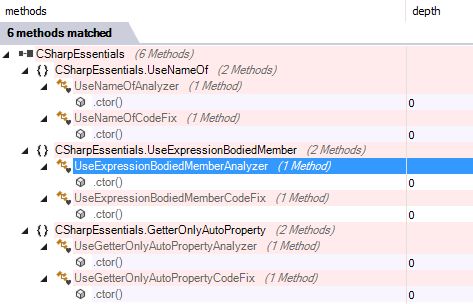
\includegraphics[width=0.8\textwidth]{images/dead-methods.png}
\caption{Potentially dead Methods}
\vspace{0.1cm}
Von NDepend gefundener wahrscheinlich nicht aufgerufener Quelltext
\label{fig:dead-methods}
\end{figure}

\subsubsection{Quelltextmetriken}
Mit Hilfe des Code Metrics View lassen sich Quelltextmetriken visualisieren. Auflösungen von Assembly über Namespaces bis Methoden stehen zur Auswahl. In größeren System, welche aus mehren Assemblies bestehen, möchte man nach kritischen Teilprogrammen suchen. Mit knapp über 1000 Quelltextzeilen und nur einer Assembly in CSharpEssentials ist die Auflösung nach Methoden am sinnvollsten. IL Nesting Depth, Cyclomatic Complexity und IL Cyclomatic Complexity erzeugen die in den Abbildungen~\ref{fig:nd-il-nesting-depth},~\ref{fig:nd-cyclomatic-complexity} und ~\ref{fig:nd-il-cyclomatic-complexity} dargestellten Code Metric Views.

\begin{figure}[ht]
	\centering
	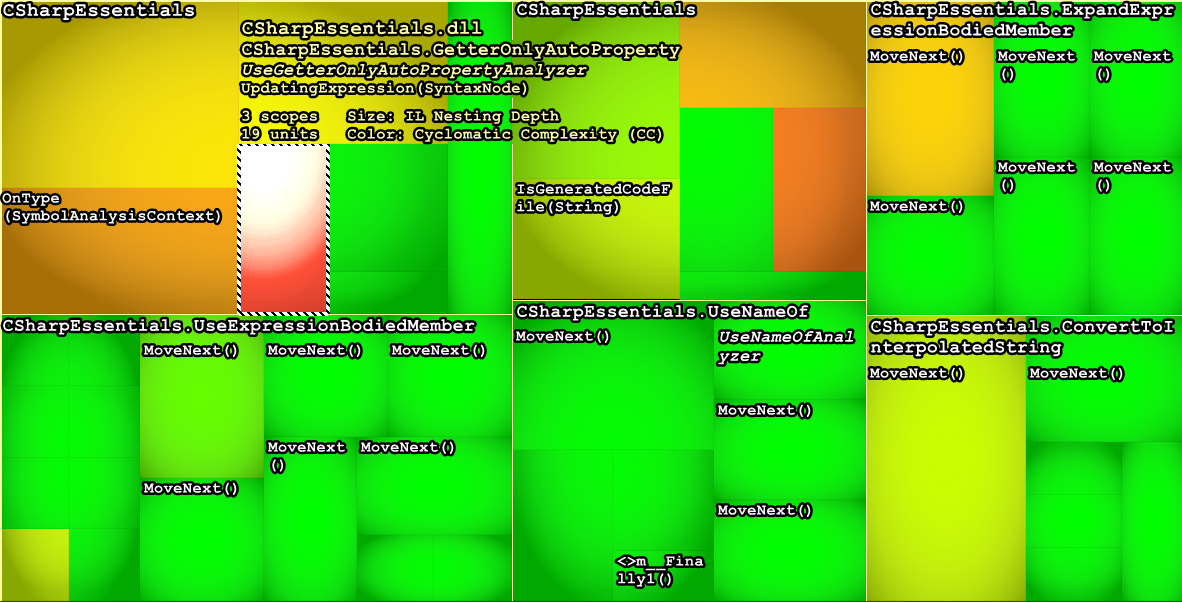
\includegraphics[width=0.8\textwidth]{images/nd-il-nesting-depth.png}
	\caption{}
	\vspace{0.1cm}
	\label{fig:nd-il-nesting-depth}
\end{figure}

\begin{figure}[ht]
	\centering
	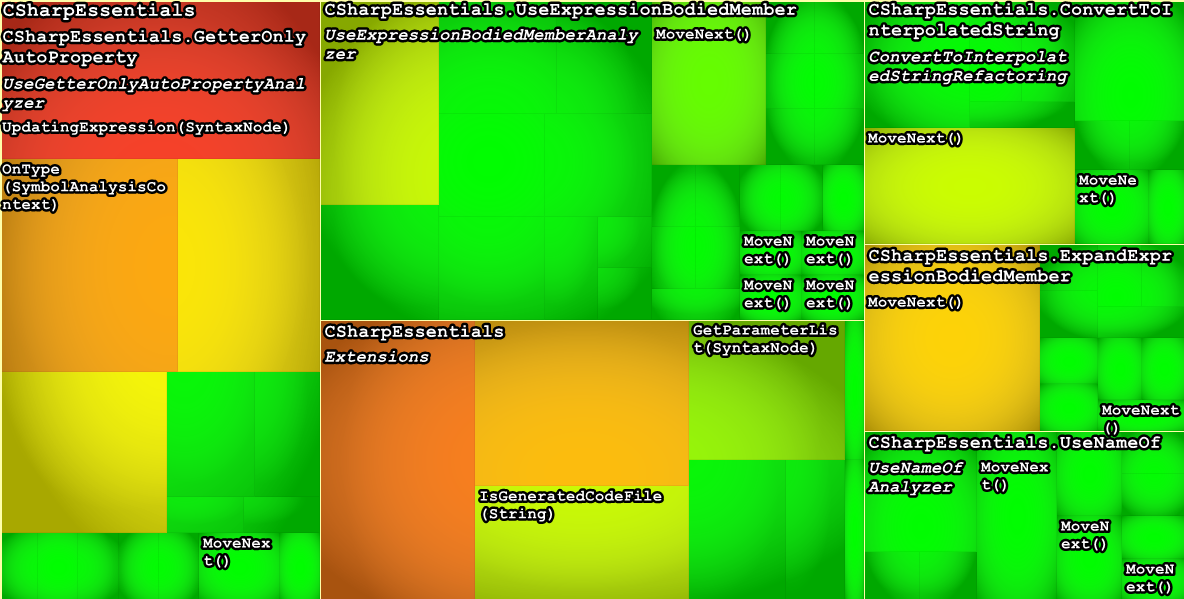
\includegraphics[width=0.8\textwidth]{images/nd-cyclomatic-complexity.png}
	\caption{}
	\vspace{0.1cm}
	\label{fig:nd-cyclomatic-complexity}
\end{figure}

\begin{figure}[ht]
	\centering
	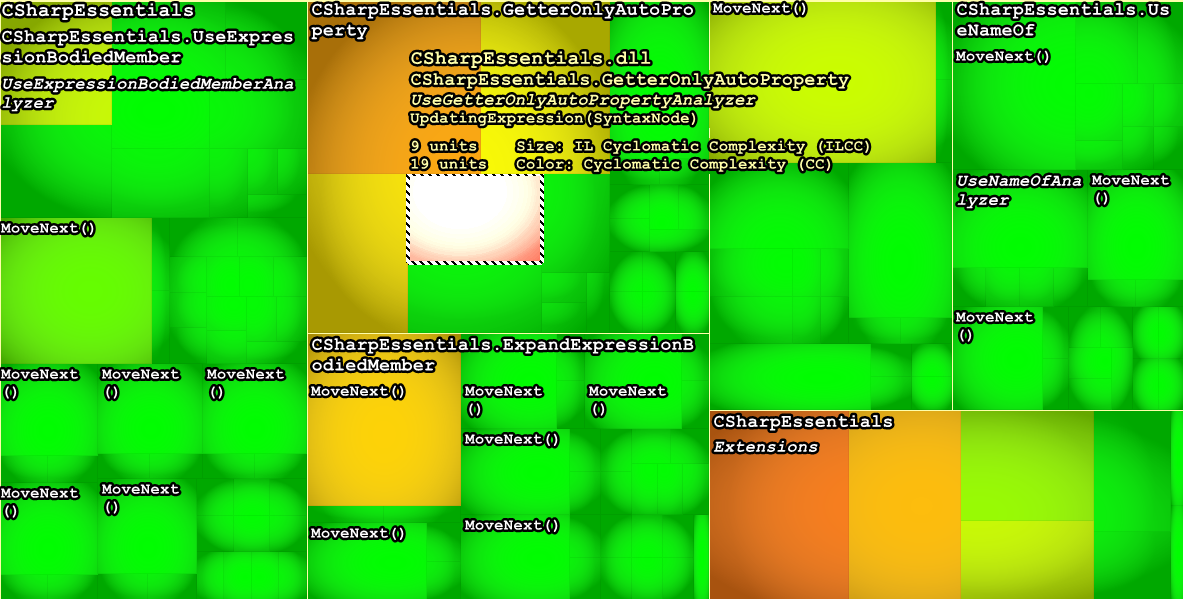
\includegraphics[width=0.8\textwidth]{images/nd-il-cyclomatic-complexity.png}
	\caption{}
	\vspace{0.1cm}
	\label{fig:nd-il-cyclomatic-complexity}
\end{figure}

\subsection{ReSharper}


\subsection{Visual Studio Tools}
Visual Studio analysiert Code, erstellt dabei Quelltextmetriken und kann zum Beispiel Code-Clone identifizieren.

\subsubsection{Quelltextmetriken}

\subsubsection{Code-Clone}


\subsection{Gendarme}
Gendarme analysiert Programme und Bibliotheken, welche in den verschiedenen .NET Sprachen geschrieben wurden. Dafür benötigt Gendarme eine kompilierte Assembly, weil es nicht den C\# statisch analysiert, sondern ein daraus erzeugte Spracheformat: Das ECMA CIL.~\cite{ecma} Die CIL wird mit Hilfe von der Bibliothek Cecil analysiert.~\cite{cecil} Gendarme generiert auf Basis dieser Analyse Berichte. Sie können als HTML-Datei exportiert werden.

\paragraph{ECMA CIL}

\subsubsection{Fehler}

\subsubsection{Sicherheiten}


\subsection{SourceMonitor}

\subsubsection{Kiviat-Chart}
